\section{\eTrice{} Models and Their Relations}

\eTrice{} comprises several models:

\begin{itemize}
\item the ROOM model (*.room) -- defines model classes and the logical structure of the model
\item the Config model (*.config) -- defines configuration values for attributes
\item the Physical model (*.etphys) -- defines the structure and properties of the physical system
\item the Mapping model (*.etmap) -- defines a mapping from logical elements to physical elements
\end{itemize}

In the following diagram the models and their relations are depicted. The meaning of the arrows is: 
uses/references.

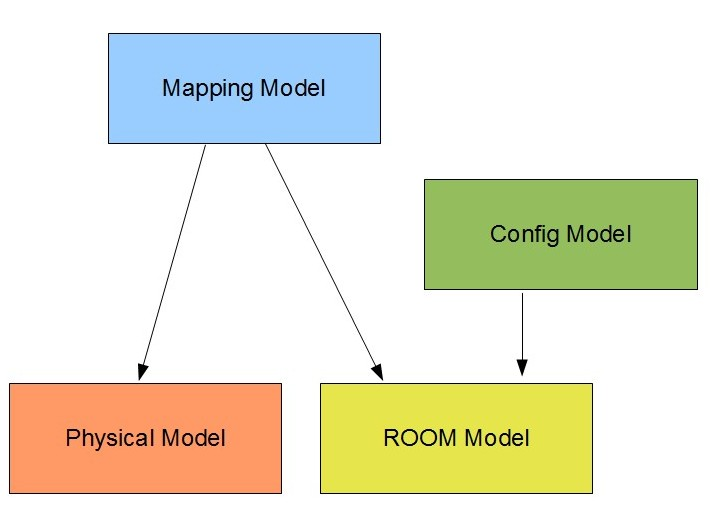
\includegraphics[scale=0.4]{images/080-models.jpg}

In the following sections we will describe those models with emphasis of their cross relations.

\subsection{The ROOM Model}

The ROOM model defines \room{DataClass}es, \room{ProtocolClass}es, \room{ActorClass}es, \room{SubSystemClass}es and \room{LogicalSystem}s.
Thereby the three latter form a hierarchy. The \room{LogicalSystem} is the top level element of the structure. 
It contains references to \room{SubSystemClass} elements. The \room{SubSystemClass} in turn contains 
references to \room{ActorClass} elements which again contain (recursively) references to 
\room{ActorClass} elements. The complete structural hierarchy implies a tree which has the 
\room{LogicalSystem} as root and where each reference stands for a new node with possibly further 
branches.

Let's consider a simple example. It doesn't implement anything meaningful and completely omits behavioral and 
other aspects.

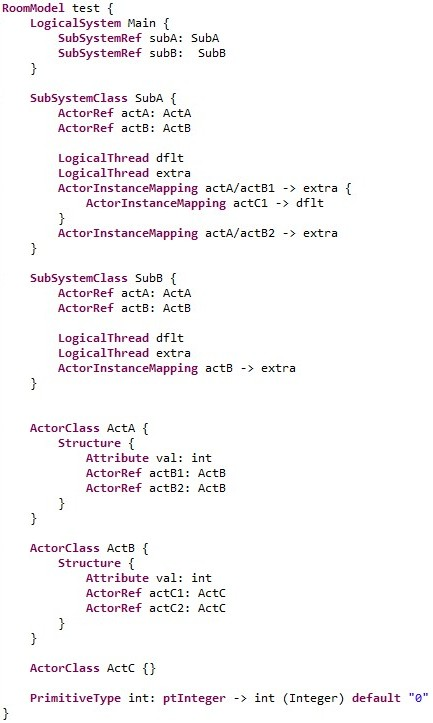
\includegraphics{images/080-room.jpg}

When a \room{LogicalSystem} is instantiated then recursively all of the contained referenced elements are 
instantiated as instances of the corresponding class. Thus the instance tree of the above example looks like 
in figure \ref{fig:instance_tree} (the third line in the white boxes shows some mapping information,
see section \ref{sec:mapping_model} \nameref{sec:mapping_model}):

\begin{figure}
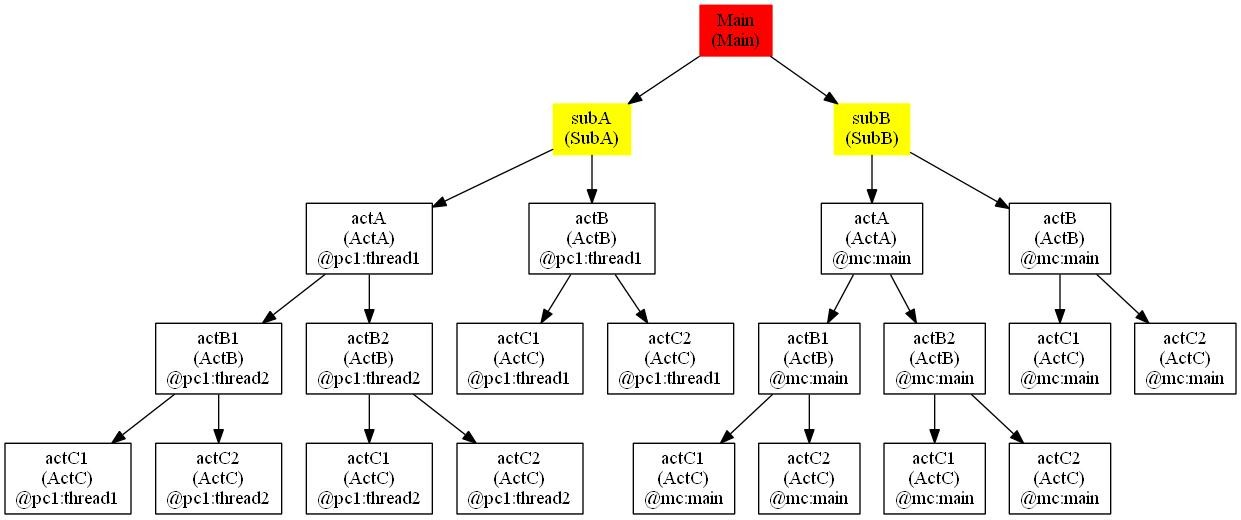
\includegraphics[scale=0.45]{images/080-instances.jpg}
\caption{Instances of a ROOM system}
\label{fig:instance_tree}
\end{figure}

Here is a long example of a ROOM file (not complete):

\begin{lstlisting}[language=ROOM]
RoomModel trafficlight.example {

	import room.basic.types.* from "../../../org.eclipse.etrice.modellib.c/model/Types.room"

	import room.basic.service.timing.* from "../../../org.eclipse.etrice.modellib.c/model/TimingService.room"

	import room.basic.service.tcp.* from "../../../org.eclipse.etrice.modellib.c/model/TcpService.room"

	LogicalSystem LSTraffic {
		SubSystemRef main: SSTraffic
	}
	
	SubSystemClass SSTraffic ["Subsystem of Trafficlight Example Application. The Subsystem contains all Actors of the application."] {
		ActorRef application: TrafficlightExampleApplication ["reference to application"]
		ActorRef TimingService: ATimingService ["reference to timing service"]
		LayerConnection ref application satisfied_by TimingService.timer 
	
		LogicalThread dflt_thread
	}

	ActorClass TrafficlightExampleApplication ["Toplevel Actor of the Trafficlight Example Application."]{
		Structure {
			
			ActorRef light1: TrafficLight ["first traffic light"]
			ActorRef light2: TrafficLight ["second traffic light"]
			ActorRef controller: TrafficController ["controller for coordination of the traffic lights"]
			Binding controller.light1 and light1.controller 
			Binding controller.light2 and light2.controller
		}
		Behavior { }
	}

	ActorClass TrafficController ["The TrafficController coordinates two traffic lights (directions)."] {
		Interface {
			conjugated Port light1: PTrafficLight ["port to control traffic light 1"]
			conjugated Port light2: PTrafficLight ["port to control traffic light 2"]
		}
		Structure {
			usercode1 {
				"#include \"platform/etTcpSockets.h\""
			}
			external Port light1 
			external Port light2 
			SAP timeout: PTimer
		}
		Behavior {
			Operation TrafficController() {
				"etInitSockets();"
			}
			Operation ~TrafficController() {
				"etCleanupSockets();"
			}
			StateMachine {
				Transition init: initial -> Idle { }
				Transition tr0: Idle -> SwitchToLight1GreenForCars {
					triggers {
						<timeout: timeout>
					}
				}
				Transition tr1: SwitchToLight1GreenForCars -> state0 {
					triggers {
						<greenForCarDone: light1>
					}
				}
				Transition tr2: SwitchToLight1GreenForCars -> state1 {
					triggers {
						<greenForPedDone: light2>
					}
				}
				Transition tr3: state1 -> Light1GreenForCars {
					triggers {
						<greenForCarDone: light1>
					}
				}
				Transition tr4: state0 -> Light1GreenForCars {
					triggers {
						<greenForPedDone: light2>
					}
				}
				Transition tr5: Light1GreenForCars -> SwitchToLight2GreenForCars {
					triggers {
						<timeout: timeout>
					}
				}
				Transition tr6: SwitchToLight2GreenForCars -> state2 {
					triggers {
						<greenForPedDone: light1>
					}
				}
				Transition tr7: SwitchToLight2GreenForCars -> state3 {
					triggers {
						<greenForCarDone: light2>
					}
				}
				Transition tr8: state2 -> Light2GreenForCars {
					triggers {
						<greenForCarDone: light2>
					}
				}
				Transition tr9: state3 -> Light2GreenForCars {
					triggers {
						<greenForPedDone: light1>
					}
				}
				Transition tr10: Light2GreenForCars -> SwitchToLight1GreenForCars {
					triggers {
						<timeout: timeout>
					}
				}
				State Idle {
					entry {
						"timeout.startTimeout(3000);"
					}
				}
				State Light1GreenForCars {
					entry {
						"timeout.startTimeout(10000);"
					}
				}
				State SwitchToLight1GreenForCars {
					entry {
						"light1.greenForCar();"
						"light2.greenForPed();"
					}
				}
				State state0
				State state1
				State SwitchToLight2GreenForCars {
					entry {
						"light1.greenForPed();"
						"light2.greenForCar();"
					}
				}
				State state2
				State state3
				State Light2GreenForCars {
					entry {
						"timeout.startTimeout(10000);"
					}
				}
			}
		}
	}
\end{lstlisting}

\subsection{The Config Model}

Once we have the ROOM class model we can configure values using the Config model. This can be done on the 
class level and/or on the instance level. Values defined for class attributes are used for all instances 
unless there is an instance value configured for the same attribute.

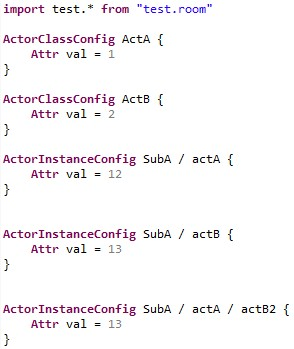
\includegraphics{images/080-config.jpg}

\begin{lstlisting}[language=Config]
ConfigModel de.protos.automation.MachineElementsTest.config {
	import de.protos.automation.MachineElementsTest.* from "MachineElementsTest.room"
	
	ActorInstanceConfig MachineElementsTestSystem/ioServiceTest/test/cylinder {
		Attr channelOutPos0 = 0
		Attr channelOutPos1 = 1
		Attr channelInPos0 = 0
		Attr channelInPos1 = 1
		Attr errorTimeoutConfig = 3000
	}
	
	ActorInstanceConfig MachineElementsTestSystem/ioServiceTest/test/cylinderSim {
		Attr channelOutPos0 = 0
		Attr channelOutPos1 = 1
		Attr channelInPos0 = 0
		Attr channelInPos1 = 1

		Attr minPosition = 0
		Attr maxPosition = 100
		Attr currentPosition = 0
		Attr stepWidth = 10
	}
}\end{lstlisting}

\subsection{The Physical Model}

The physical model defines the physical resources onto which the logical system will be deployed. It is 
possible to define runtime classes which (currently) only define the overall execution model of the 
platform.

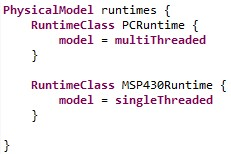
\includegraphics{images/080-runtimes.jpg}

The \room{PhysicalSystem} is composed of \room{NodeRef}erences which are instances
of \room{NodeClass}es. Each \room{NodeClass} os referencing a 
\room{RuntimeClass} and is defining \room{Threads}.

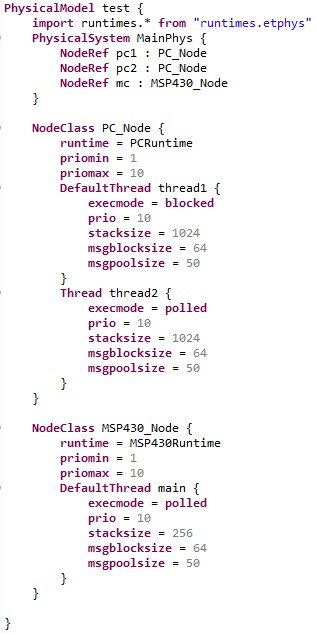
\includegraphics{images/080-phys.jpg}

\begin{lstlisting}[language=etPhys]
PhysicalModel cGenRef {

	PhysicalSystem Sys {
		NodeRef node1: PC
		NodeRef node2: PC
	}
	
	NodeClass PC {
		runtime = PC
		priomin = 1
		priomax = 5
		
		DefaultThread PhysicalThread1 {
			execmode = blocked
			prio = 5
			stacksize = 1024
			msgblocksize = 64
			msgpoolsize = 256
		}
		
		Thread PhysicalThread2 {
			execmode = blocked
			prio = 5
			stacksize = 1024
			msgblocksize = 64
			msgpoolsize = 256
		}
	}
	
	RuntimeClass PC {
		model = multiThreaded
	}
}
\end{lstlisting}

\subsection{The Mapping Model}
\label{sec:mapping_model}

The last model finally combines all this information by mapping logical to physical entities.

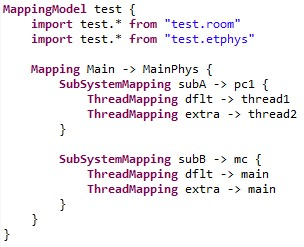
\includegraphics{images/080-map.jpg}

\begin{lstlisting}[language=etMap]
MappingModel cgenRef {
	
	import cGenRef from "cGenRef.room"
	import cGenRef from "cGenRef.etphys"
	
	Mapping cGenRef.LS -> cGenRef.Sys {
		SubSystemMapping sys1 -> node1 {
			ThreadMapping dflt_thread -> PhysicalThread1
			ThreadMapping other_thread -> PhysicalThread2
		}
		SubSystemMapping sys2 -> node2 {
			ThreadMapping dflt_thread -> PhysicalThread1
			ThreadMapping other_thread -> PhysicalThread2
		}
	}
}
\end{lstlisting}

The result of the mapping is also depicted in above tree diagram (figure \ref{fig:instance_tree})
of the instances. All actor instances (the white boxes) are mapped to a node and a thread running on this node
(shown as @\textit{node} : \textit{thread}).

